
%----------------------------------------------------------------------------------------
%    PACKAGES AND THEMES  (template: SimpleDarkBlue, as in your Lecture2.tex)
%----------------------------------------------------------------------------------------
\documentclass[aspectratio=169,xcolor=dvipsnames]{beamer}
\usetheme{SimpleDarkBlue}

\usepackage{hyperref}
\usepackage{graphicx}
\usepackage{booktabs}
\usepackage{amsmath,amssymb,mathtools}

\usepackage{fontspec}
\usepackage{luatexja}
\usepackage{appendixnumberbeamer}

\setmainfont{Alegreya Sans Light}[
  ItalicFont={* Italic},
  BoldFont={Alegreya Sans Medium},
  BoldItalicFont={Alegreya Sans Medium Italic}]
\setsansfont{Alegreya Sans Light}[
  ItalicFont={* Italic},
  BoldFont={Alegreya Sans Medium},
  BoldItalicFont={Alegreya Sans Medium Italic}]

% ------------------------------------ %
% Section title page with Huge bf text %
% ------------------------------------ %
\AtBeginSection[]{
  \begin{frame}[noframenumbering, plain]
    \Huge{\centerline{\textbf{\insertsection}}}
  \end{frame}
}

%%% automatically add spaces into enumerate and itemize environment
\let\tempone\itemize
\let\temptwo\enditemize
\renewenvironment{itemize}{\tempone\addtolength{\itemsep}{\fill}}{\temptwo}
\let\tempa\enumerate
\let\tempb\endenumerate
\renewenvironment{enumerate}{\tempa\addtolength{\itemsep}{\fill}}{\tempb}

% --- Footline (copied style from Lecture2.tex) ---
\defbeamertemplate*{footline}{shadow theme}{%
    \leavevmode\hbox{%
        \hypersetup{linkcolor=white,urlcolor=white,citecolor=white}
        \begin{beamercolorbox}[wd=1.02\paperwidth, ht=2.5ex, dp=1.125ex, leftskip=.3cm plus1fil, rightskip=0.3cm]{author in head/foot}%
            \insertsectionnavigationhorizontal{.80\textwidth}{}{} \hspace{.3cm} \hfill \#\ \insertframenumber \ / \ \inserttotalframenumber%
        \end{beamercolorbox}%
    }%
}
\setbeamertemplate{footline}[shadow theme]
\setbeamertemplate{navigation symbols}{}

% --- color helpers (in case theme doesn't define them) ---
\providecommand{\blue}[1]{\textcolor{RoyalBlue}{#1}}
\providecommand{\red}[1]{\textcolor{BrickRed}{#1}}

%----------------------------------------------------------------------------------------
%    TITLE PAGE
%----------------------------------------------------------------------------------------
\title[RBC 1A]{RBC Topic 1A: Business-Cycle Facts and the HP Filter}
\author[Hui-Jun Chen]{Hui-Jun Chen}
\institute[]{National Tsing Hua University\\ Department of Economics}
\date{\today}

\begin{document}

\begin{frame}[plain,noframenumbering]
    \titlepage
\end{frame}

%========================================================================================
\section{Business-Cycle Facts}
%========================================================================================

\begin{frame}{The recent U.S. recession: unfiltered first look}
\label{slide:Topic1A_Unfiltered}
\centering
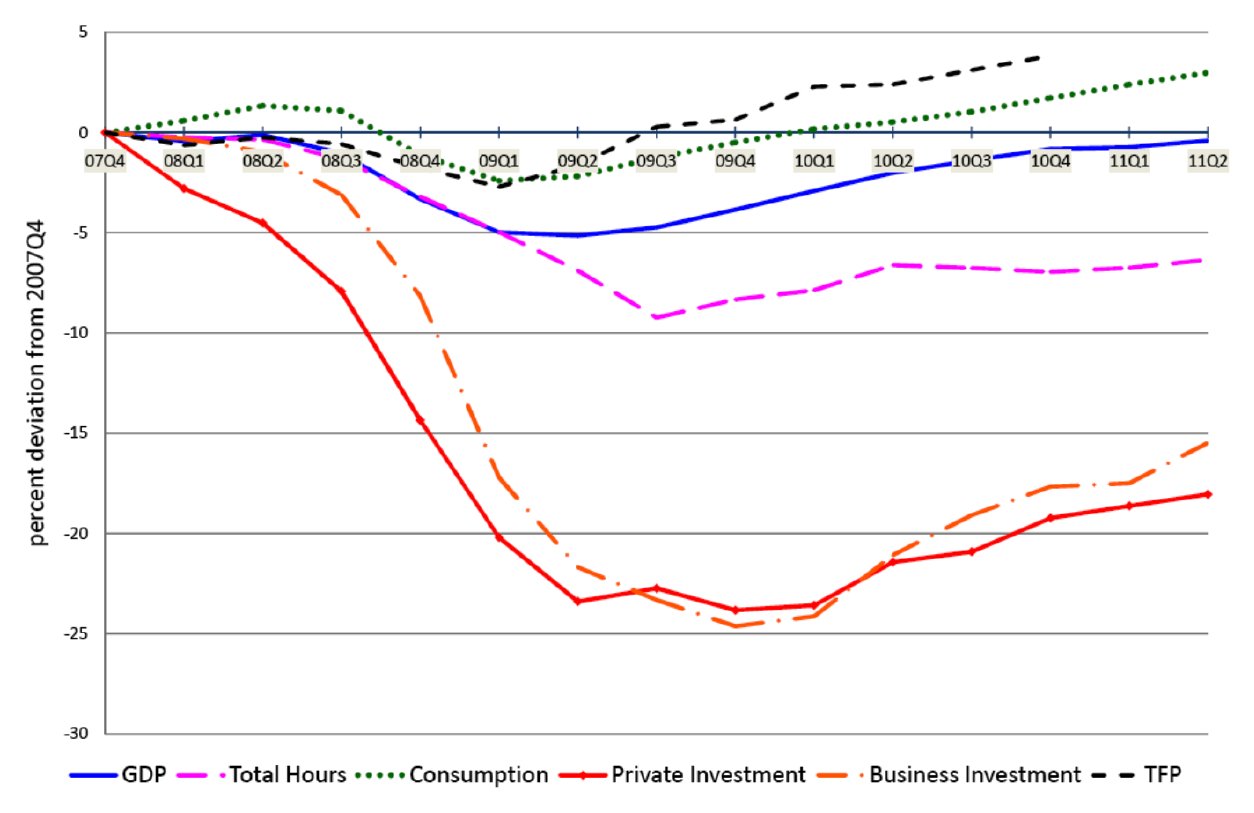
\includegraphics[width=0.8\textwidth]{topic1_figs/topic1_p01.png}
\end{frame}

\begin{frame}{The recent U.S. recession: HP-filtered data}
\label{slide:Topic1A_HPfiltered}
\centering
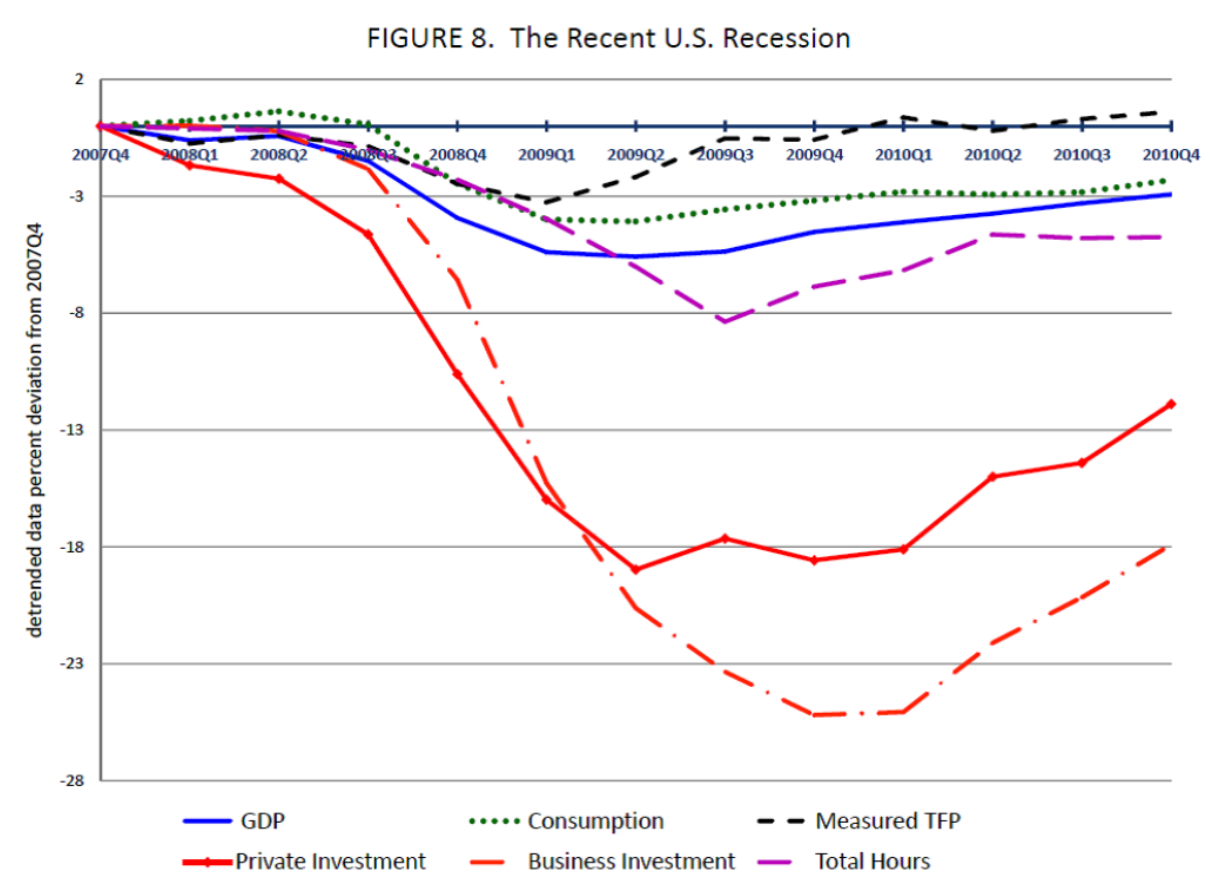
\includegraphics[width=0.7\textwidth]{topic1_figs/topic1_p02.png}
\end{frame}

\begin{frame}{Basic business cycle facts (stylized)}
\label{slide:Topic1A_FactsTable}
\centering
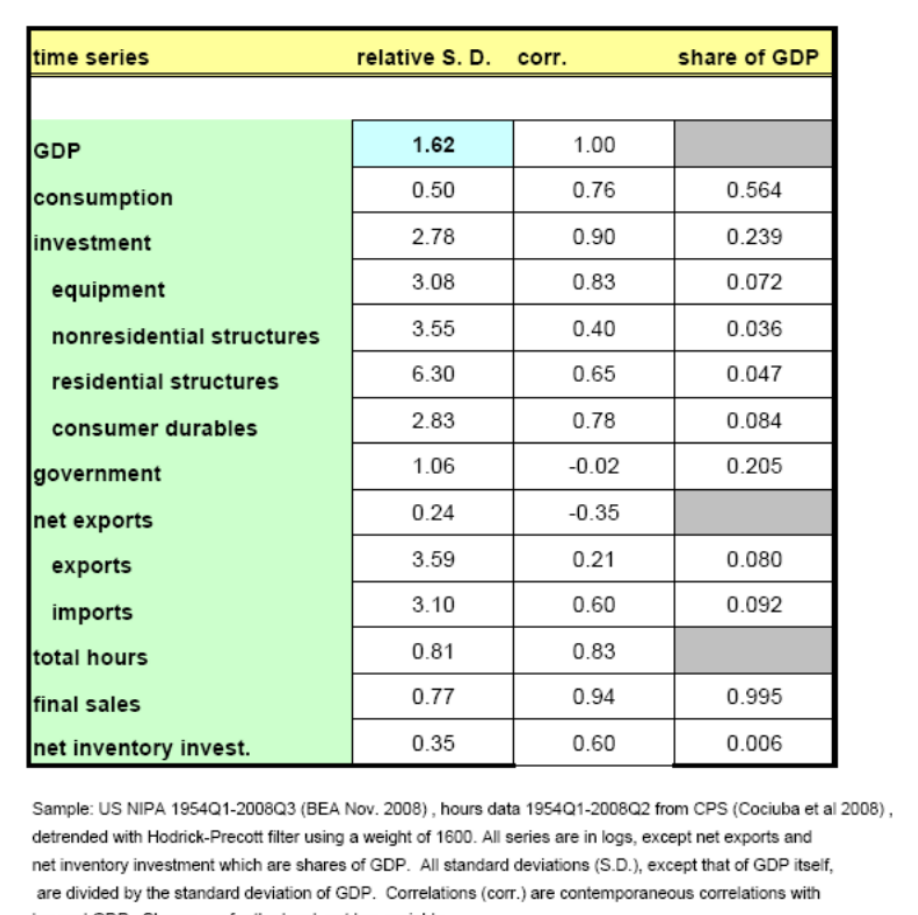
\includegraphics[width=0.65\textwidth]{topic1_figs/topic1_p03.png}
\end{frame}

\begin{frame}{Basic business cycle facts: detrended GDP, consumption, investment}
\label{slide:Topic1A_FactsSeries}
\centering
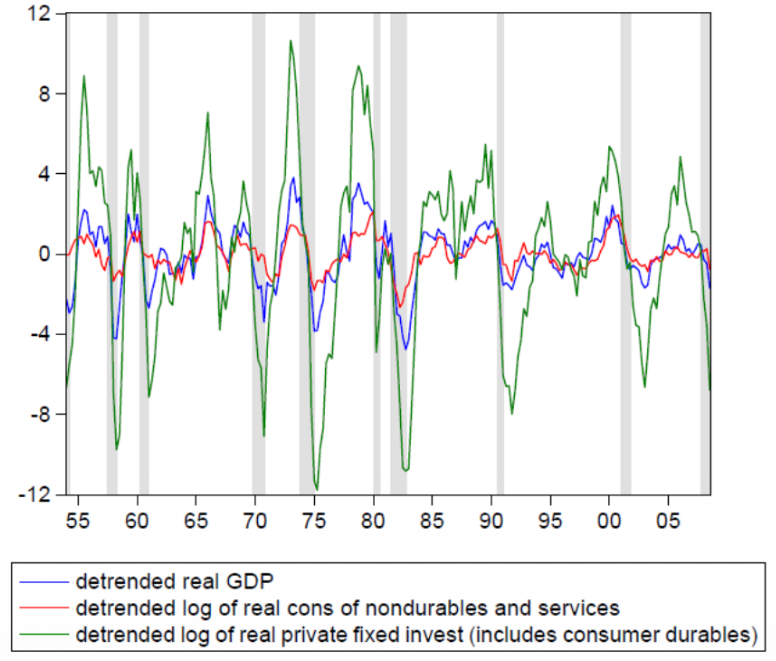
\includegraphics[width=0.6\textwidth]{topic1_figs/topic1_p04.png}
\end{frame}

\begin{frame}{Where we are going in RBC}
\label{slide:Topic1A_Outline}
\small
\begin{enumerate}
    \item \blue{Detrend the data}: Hodrick--Prescott (HP) filter
    \item \blue{Growth in the model}: exogenous technical progress
    \begin{enumerate}
        \item Characterize the balanced growth path (BGP)
        \item Growth-deflate to study stationary series
    \end{enumerate}
    \item \blue{Calibrate} steady state to long-run data (preview)
    \item \blue{Solve} the growth-deflated model (we postpone linearization / KPR methods)
\end{enumerate}

\vspace{0.4em}
\textbf{Goal for today:} Learn how we measure ``cycles'' in data (HP filter), then build a model that can speak to these facts.
\end{frame}

%========================================================================================
\section{HP Filter}
%========================================================================================

\begin{frame}{Postwar U.S. GDP and its HP trend}
\label{slide:Topic1A_GDPTrendFig}
\centering
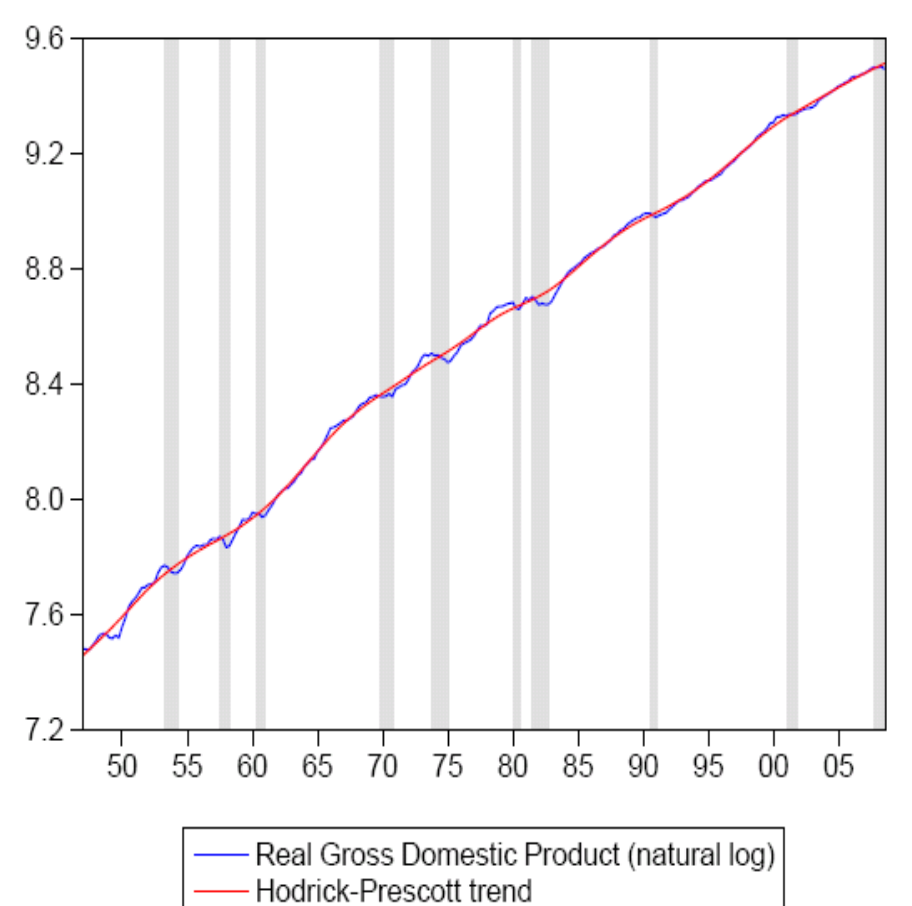
\includegraphics[width=0.5\textwidth]{topic1_figs/topic1_p06.png}
\end{frame}

\begin{frame}{HP filter: the minimization problem}
\label{slide:Topic1A_HP_Def}
\small
Given data \(\{y_t\}_{t=1}^T\), the HP filter chooses a trend \(\{\tau_t\}_{t=1}^T\) by
\[
\min_{\{\tau_t\}_{t=1}^T}\;
\frac{1}{T}\sum_{t=1}^{T}(y_t-\tau_t)^2
\;+\;
\frac{\lambda}{T-1}\sum_{t=2}^{T-1}
\Big[(\tau_{t+1}-\tau_t)-(\tau_t-\tau_{t-1})\Big]^2,
\tag{HP}
\]
where \(\lambda>0\) controls smoothness.

\begin{itemize}
    \item First term: \blue{fit} (trend close to data).
    \item Second term: \blue{smoothness} (penalize changes in trend growth; a second-difference penalty).
    \item Detrended (cycle) series: \(\tilde y_t \equiv y_t-\tau_t\).
\end{itemize}
\end{frame}

\begin{frame}{How \(\lambda\) affects the identified HP trend}
\label{slide:Topic1A_LambdaTrend}
\centering
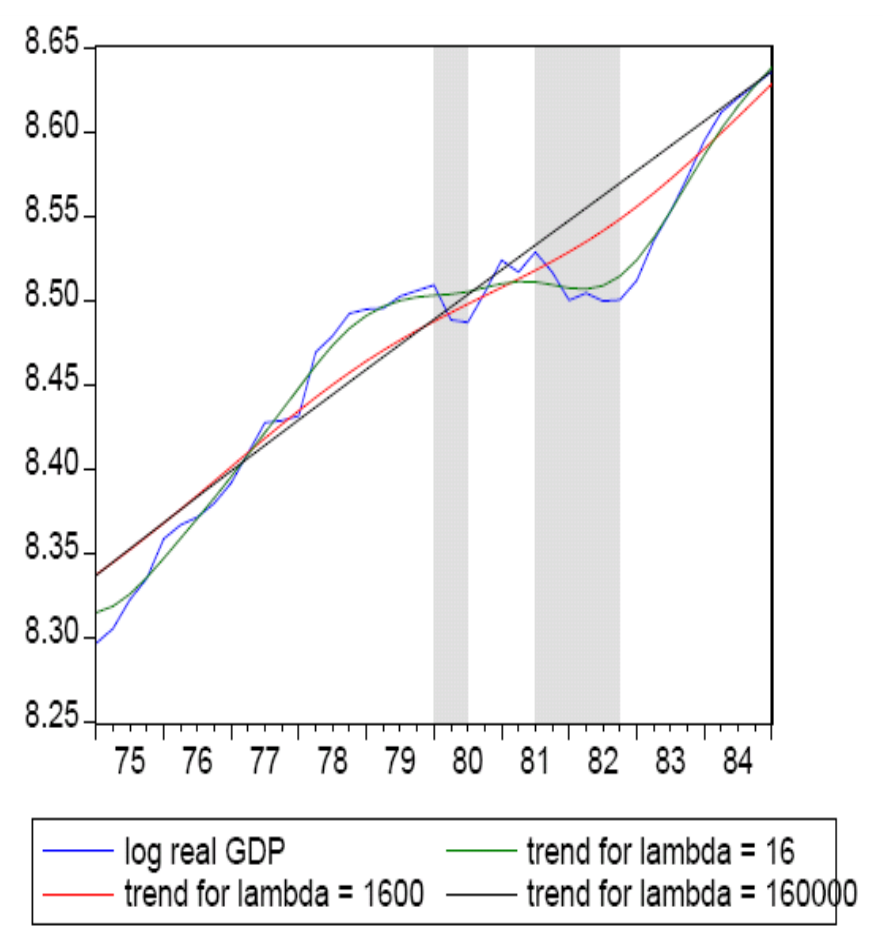
\includegraphics[width=0.5\textwidth]{topic1_figs/topic1_p08.png}
\end{frame}

\begin{frame}{How \(\lambda\) affects identified business cycles}
\label{slide:Topic1A_LambdaCycle}
\centering
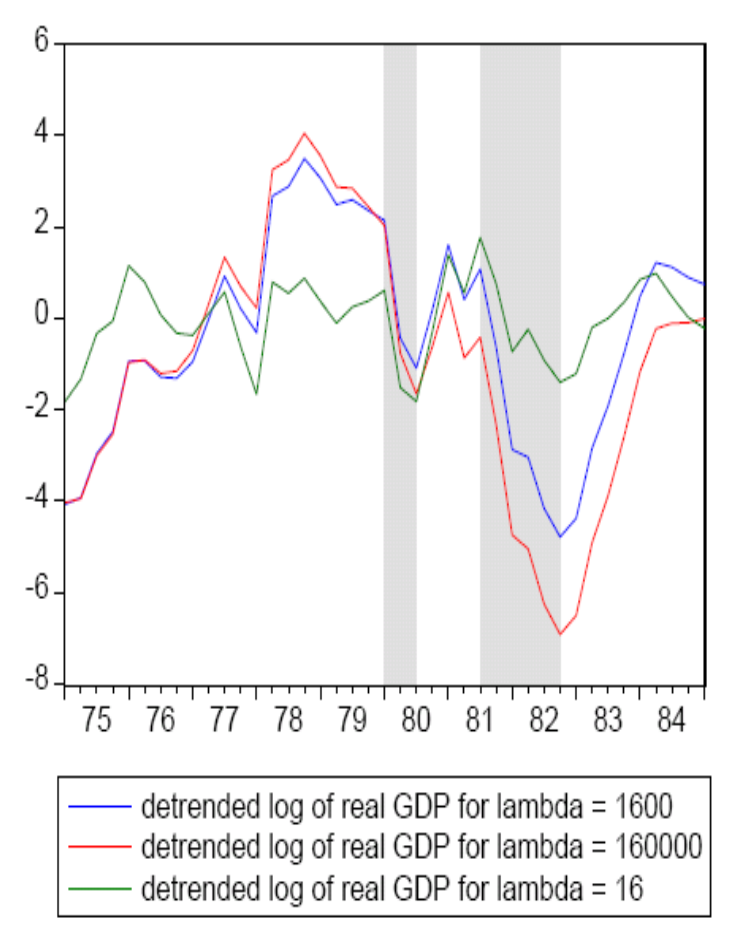
\includegraphics[width=0.4\textwidth]{topic1_figs/topic1_p09.png}
\end{frame}

\begin{frame}{HP objective expanded: see where FOCs come from}
\label{slide:Topic1A_ObjectiveExpanded}
\footnotesize
The objective is a quadratic function of \((\tau_1,\ldots,\tau_T)\):
\[
\sum_{t=1}^T (y_t-\tau_t)^2
\;+\;
\lambda\sum_{t=2}^{T-1}\big(\tau_{t+1}-2\tau_t+\tau_{t-1}\big)^2.
\]
The penalty term uses the \blue{second difference} \(\Delta^2\tau_t \equiv \tau_{t+1}-2\tau_t+\tau_{t-1}\).

\vspace{0.3em}
\textbf{Generic interior FOC idea:} for \(2<t<T-1\), \(\tau_t\) appears in \((y_t-\tau_t)^2\) and in three nearby penalty terms:
\(\Delta^2\tau_{t-1}\), \(\Delta^2\tau_t\), \(\Delta^2\tau_{t+1}\).
\end{frame}

\begin{frame}{The ordinary first-order condition (interior dates)}
\label{slide:Topic1A_FOC_Interior}
\footnotesize
For an interior date \(t\) with \(2<t<T-1\), the FOC is a \blue{linear difference equation} involving
\(\tau_{t-2},\tau_{t-1},\tau_t,\tau_{t+1},\tau_{t+2}\):
\[
2(y_t-\tau_t)
+2\lambda\Big[
(\tau_t-\tau_{t-1})-(\tau_{t-1}-\tau_{t-2})
-2\big((\tau_{t+1}-\tau_t)-(\tau_t-\tau_{t-1})\big)
+(\tau_{t+2}-\tau_{t+1})-(\tau_{t+1}-\tau_t)
\Big]=0.
\]
\begin{itemize}
    \item This is a \blue{fifth-order} linear difference equation (uses \(\tau_{t-2}\) through \(\tau_{t+2}\)).
    \item Endpoint dates have ``missing'' terms and hence different FOCs.
\end{itemize}
\end{frame}

\begin{frame}{Endpoint terms: why first and last dates differ}
\label{slide:Topic1A_EndPoints}
\small
At \(t=1,2,T-1,T\), some second-difference terms do not exist, so the FOCs change.

\begin{itemize}
    \item Example intuition: \(\tau_1\) only shows up in \((y_1-\tau_1)^2\) and \(\Delta^2\tau_2\) (not in \(\Delta^2\tau_0\)).
    \item Similarly, \(\tau_T\) only shows up in \((y_T-\tau_T)^2\) and \(\Delta^2\tau_{T-1}\).
\end{itemize}

\vspace{0.4em}
\textbf{Takeaway:} HP filtering is a \blue{global} smoothing problem; endpoints are special.
\end{frame}

\begin{frame}{HP filter as a linear system: \(\;y=A\tau\)}
\label{slide:Topic1A_LinearSystem}
\footnotesize
Because the objective is quadratic, the necessary and sufficient conditions are a linear system:
\[
y = A\tau,
\quad y\equiv[y_1,\ldots,y_T]^\top,\quad \tau\equiv[\tau_1,\ldots,\tau_T]^\top.
\]
The matrix \(A\) is \blue{symmetric banded} (nonzero elements on 5 diagonals). Its interior pattern is:
\[
A_{t,t} = 6\lambda+1,\quad
A_{t,t\pm1} = -4\lambda,\quad
A_{t,t\pm2} = \lambda,\qquad (2<t<T-1),
\]
with modified coefficients near the endpoints.

\medskip
\textbf{Compute:} \(\tau=A^{-1}y\), then detrend by \(\tilde y = y-\tau\).
\end{frame}

\end{document}
